\chapter{INTRODUCCIÓN}
\label{ch:1}

% Descripción de los objetivos del aprendizaje adversario:
\section{Introducción}

El objetivo principal de este trabajo es el análisis en el campo de la inteligencia artificial (\acrshort{AI}) de los distintos tipos de ataques y defensas que se pueden aplicar a un proceso de aprendizaje automático \gls{ML} de las redes neuronales, nos centraremos principalmente en el aprendizaje profundo \gls{DL}.
Este trabajo tratará principalmente de clasificar y explorar la seguridad que cuentan los modelos actuales.
Se han desarrollado una gran cantidad de modelos en los últimos años y existen una gran variedad de modelos muy distintos, aunque podemos clasificar los ataques de todos estos modelos en las siguientes categorías (evadir, envenenar, inferir o extraer).

Debemos comprender que la seguridad repercute en todo el proceso de creación y uso del modelo, desde la recogida de los datos, tratamiento, diseño, creación y ejecución del modelo.
Un ataque puede estar dirigido al conjunto de datos con el que se entrenará el modelo, a la arquitectura de la red neuronal, a los pesos, etc.
Además, un ataque puede dirigirse a descubrir muestras que produzcan resultados erróneos, por lo que los posibles vectores de ataque son muy variados y complejos.

La idea de hacer robustos los modelos es que las defensas detecten ataques a la vez que se mejora la solidez del aprendizaje, para no cometer fallos al introducir valores anómalos.

Cada uno de estos tipos de ataques tiene su nomenclatura y se debe definirse correctamente, ya que de lo contrario puede ser muy ambiguo el tipo de ataque que se está realizando, el objetivo que busca el ataque y los métodos que están empleando.

Lo que buscaremos en este trabajo será definir, analizar y estructurar los distintos tipos de ataques y sus posibles defensas, con el objetivo final de detectar y defender los modelos para hacerlos más robustos y confiables para la ciudadanía.
Además de la creación de una guía que pueda orientar a modelos más seguros y éticos.

\section{Motivación}

En la última década, se han logrado significativos avances en el campo de la inteligencia artificial. Sin embargo, a lo largo de este proceso, como suele ser habitual, se ha descuidado  aspectos cruciales relacionados con la seguridad. Esto ha dado lugar a la creación de productos que implementan la inteligencia artificial, pero presentan vulnerabilidades, riesgos potenciales, como redes neuronales poco robustas, filtraciones de datos, incumplimiento normativo, modelos que presentaban respuestas ofensivas, discriminantes ante etnias, etc. Además de presentar poca o ninguna explicabilidad de los resultados que presentan.

Esto lleva a muchas amenazas y riesgos que pueden afectar a empresas u organizaciones que apliquen inteligencia artificial si no hacen una implementación adecuada.

Problemas de seguridad en inteligencia artificial.

\begin{itemize}
    \item Alineación de la inteligencia artificial.
    \item Recopilación de datos.
    \item Bias y discriminación.
    \item Modelos poco robustos.
    \item Transparencia y explicabilidad.
    \item Escala de los modelos.
    \item Cumplimiento legal y normativo.
    \item Actualización continua.
    \item Detección de usos malintencionados.
\end{itemize}

Esto ha llevado a la creación de regulaciones de la inteligencia artificial que son muy vagas en sus conceptos de implementación.
Una primera aproximación fue el libro blanco\footnote{Se conoce como libros blancos a los documentos que publican los gobiernos en determinados casos para informar a los órganos legislativos o a la opinión pública con el objetivo de ayudar a los lectores a comprender un tema, resolver o afrontar un problema (por ejemplo diseñando una política gubernamental a largo plazo), o tomar una decisión. \href{https://es.wikipedia.org/wiki/Libro_blanco}{Enlace.}} de la inteligencia artificial en 2018 \cite{whitebook2020AI}

En este trabajo propondremos una guía similar a la matriz, \gls{MITRE-ATLAS} con buenas prácticas para la construcción de modelos más robustos y que cumplan con nuestros estándares.

% https://ec.europa.eu/commission/presscorner/detail/en/ip_23_6473
La necesidad de desarrollar un marco de inteligencia artificial fiable para todos los miembros de la Unión Europea llevo a la Comisión Europea a la creación de nuevas normativas con un enfoque basado en el \textbf{riesgo}.

Por lo que exploraremos el análisis de seguridad y posibles riesgos que se pueden dar en la sociedad.

\section{Metodología y planificación del proyecto}

Una vez definidos los objetivos del tema de investigación y desarrollo, deberemos definir el alcance para estimar el tiempo requerido y el presupuesto para el proyecto.
Recordemos que en la investigación puede ser del tipo exploratorio, buscando nuevos campos para alcanzar nuevos logros técnicos, confirmatoria para validar los resultados obtenidos en otras investigaciones o desarrollos, también puede ser una combinación de los tipos mencionados previamente.
En nuestro caso, se tratará de un proyecto híbrido, tanto de exploración como de confirmación.

% Haremos un repaso breve de las metodologías que recomienda la bibliografía existente, recordemos que las metodologías más comunes en las áreas de las ingenierías es una metodología cuantitativa.

\subsection{Metodología}

% TODO

\subsection{Planificación}

Se ha de hacer una planificación estricta de las tareas, objetivos, hitos y dependencias, para ello usaremos los diagramas Gantt\footnote{Representación gráfica de la evolución de un proyecto. \href{https://asana.com/es/resources/gantt-chart-basics}{ASANA}} con el objetivo de representar los hitos de esta investigación y del proyecto.
Seguiremos una metodología \textit{Scrum} y \textit{Lean} fijando reuniones cada semana para tener un control sobre el avance de la investigación y el desarrollo de este proyecto.

Se ha definido en la Figura \ref{fig:gantt} la lista de tareas, fecha de inicio, duración, fecha de fin y el coste de trabajo usando la técnica de tallas de camisetas.


\begin{figure}[H]
    \centering
    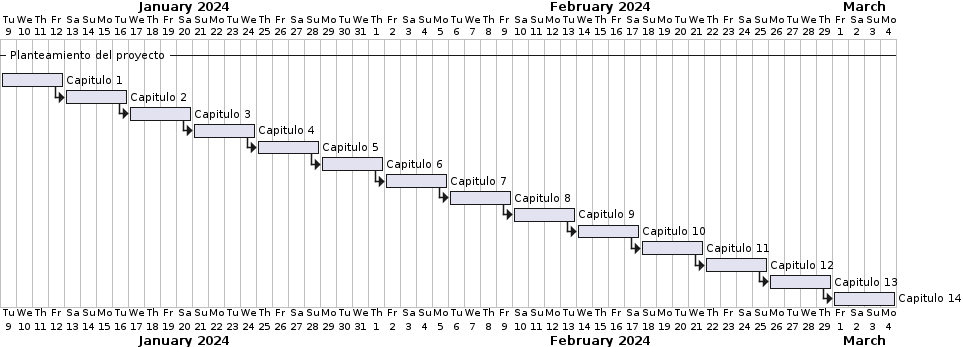
\includegraphics[width=1\linewidth]{figures/chapter01/Gantt.png}
    \caption{Diagrama Gantt}
    \label{fig:gantt}
\end{figure}
% TODO

\subsection{Presupuesto}

% TODO  


\section{Estructura de la memoria}

% En este trabajo, hemos utilizado la documentación proporcionada por \textbf{PyTorch} para explicar diversos conceptos de las redes neuronales. Nos referimos a la documentación oficial de PyTorch \cite{pytorch2024github}. Usamos el término \texttt{torch}, \texttt{torch.nn} y \texttt{nn}.

% TODO